\subsection{Der Hauptsatz der Differential- und Integralrechnung}

% In Aufgaben 48 im Buch haben wir mit geometrischen Überlegungen einige Integralfunktionen hergeleitet:
% \begin{itemize}
%     \item $F_0(x) = \int_0^x 1 \,dt = x$
%     \item $F_0(x) = \int_0^x t \,dt = \frac{1}{2}t^2$
%     \item $F_0(x) = \int_0^x (t+1) \,dt = \frac{1}{2}t^2 + t$
%     \item $F_0(x) = \int_0^x 2 \,dt = 2x$
%     \item $F_0(x) = \int_0^x 2t \,dt = t^2$
%     \item $F_0(x) = \int_0^x (2t+1) \,dt = t^2 + t$
% \end{itemize}
% In Aufgabe 49 haben wir einige andere Integralfunktionen als Grenzwerte von Ober- und Untersummen gefunden:
% \begin{itemize}
%     \item $F_0(x) = \int_0^x t^2 \,dt = \frac{1}{3}t^3$
%     \item $F_0(x) = \int_0^x t^3 \,dt = \frac{1}{4}t^4$
%     \item $F_0(x) = \int_0^x t^5 \,dt = \frac{1}{6}t^6$
%     \item $F_0(x) = \int_0^x \left(\frac{1}{2} t^2 +1 \right) \,dt = \frac{1}{6} t^3 +t$
% \end{itemize}

Bestimmte Integrale lassen sich immer als Grenzwerte von Ober- und Untersumme bestimmen. Das Problem ist aber: Diese Berechnung ist aufwendig - insbesondere weil sie für jede neue Funktion und für jedes neue Intervall von vorne begonnen werden muss.

Integralfunktionen lösen einen Teil des Problems: Kennt man von einer Funktion $f$, eine Integralfunktion $F_a(b)=\int_a^b f(x) \,dx$, kann man damit jedes bestimmte Integral von $f$ wie folgt berechnen:
$$ \int_c^d f(x) \,dx = \int_a^d f(x) \,dx - \int_a^c f(x) \,dx =F_a(d) - F_a(c)$$

\begin{figure}[!htb]
	\minipage{0.32\textwidth}
	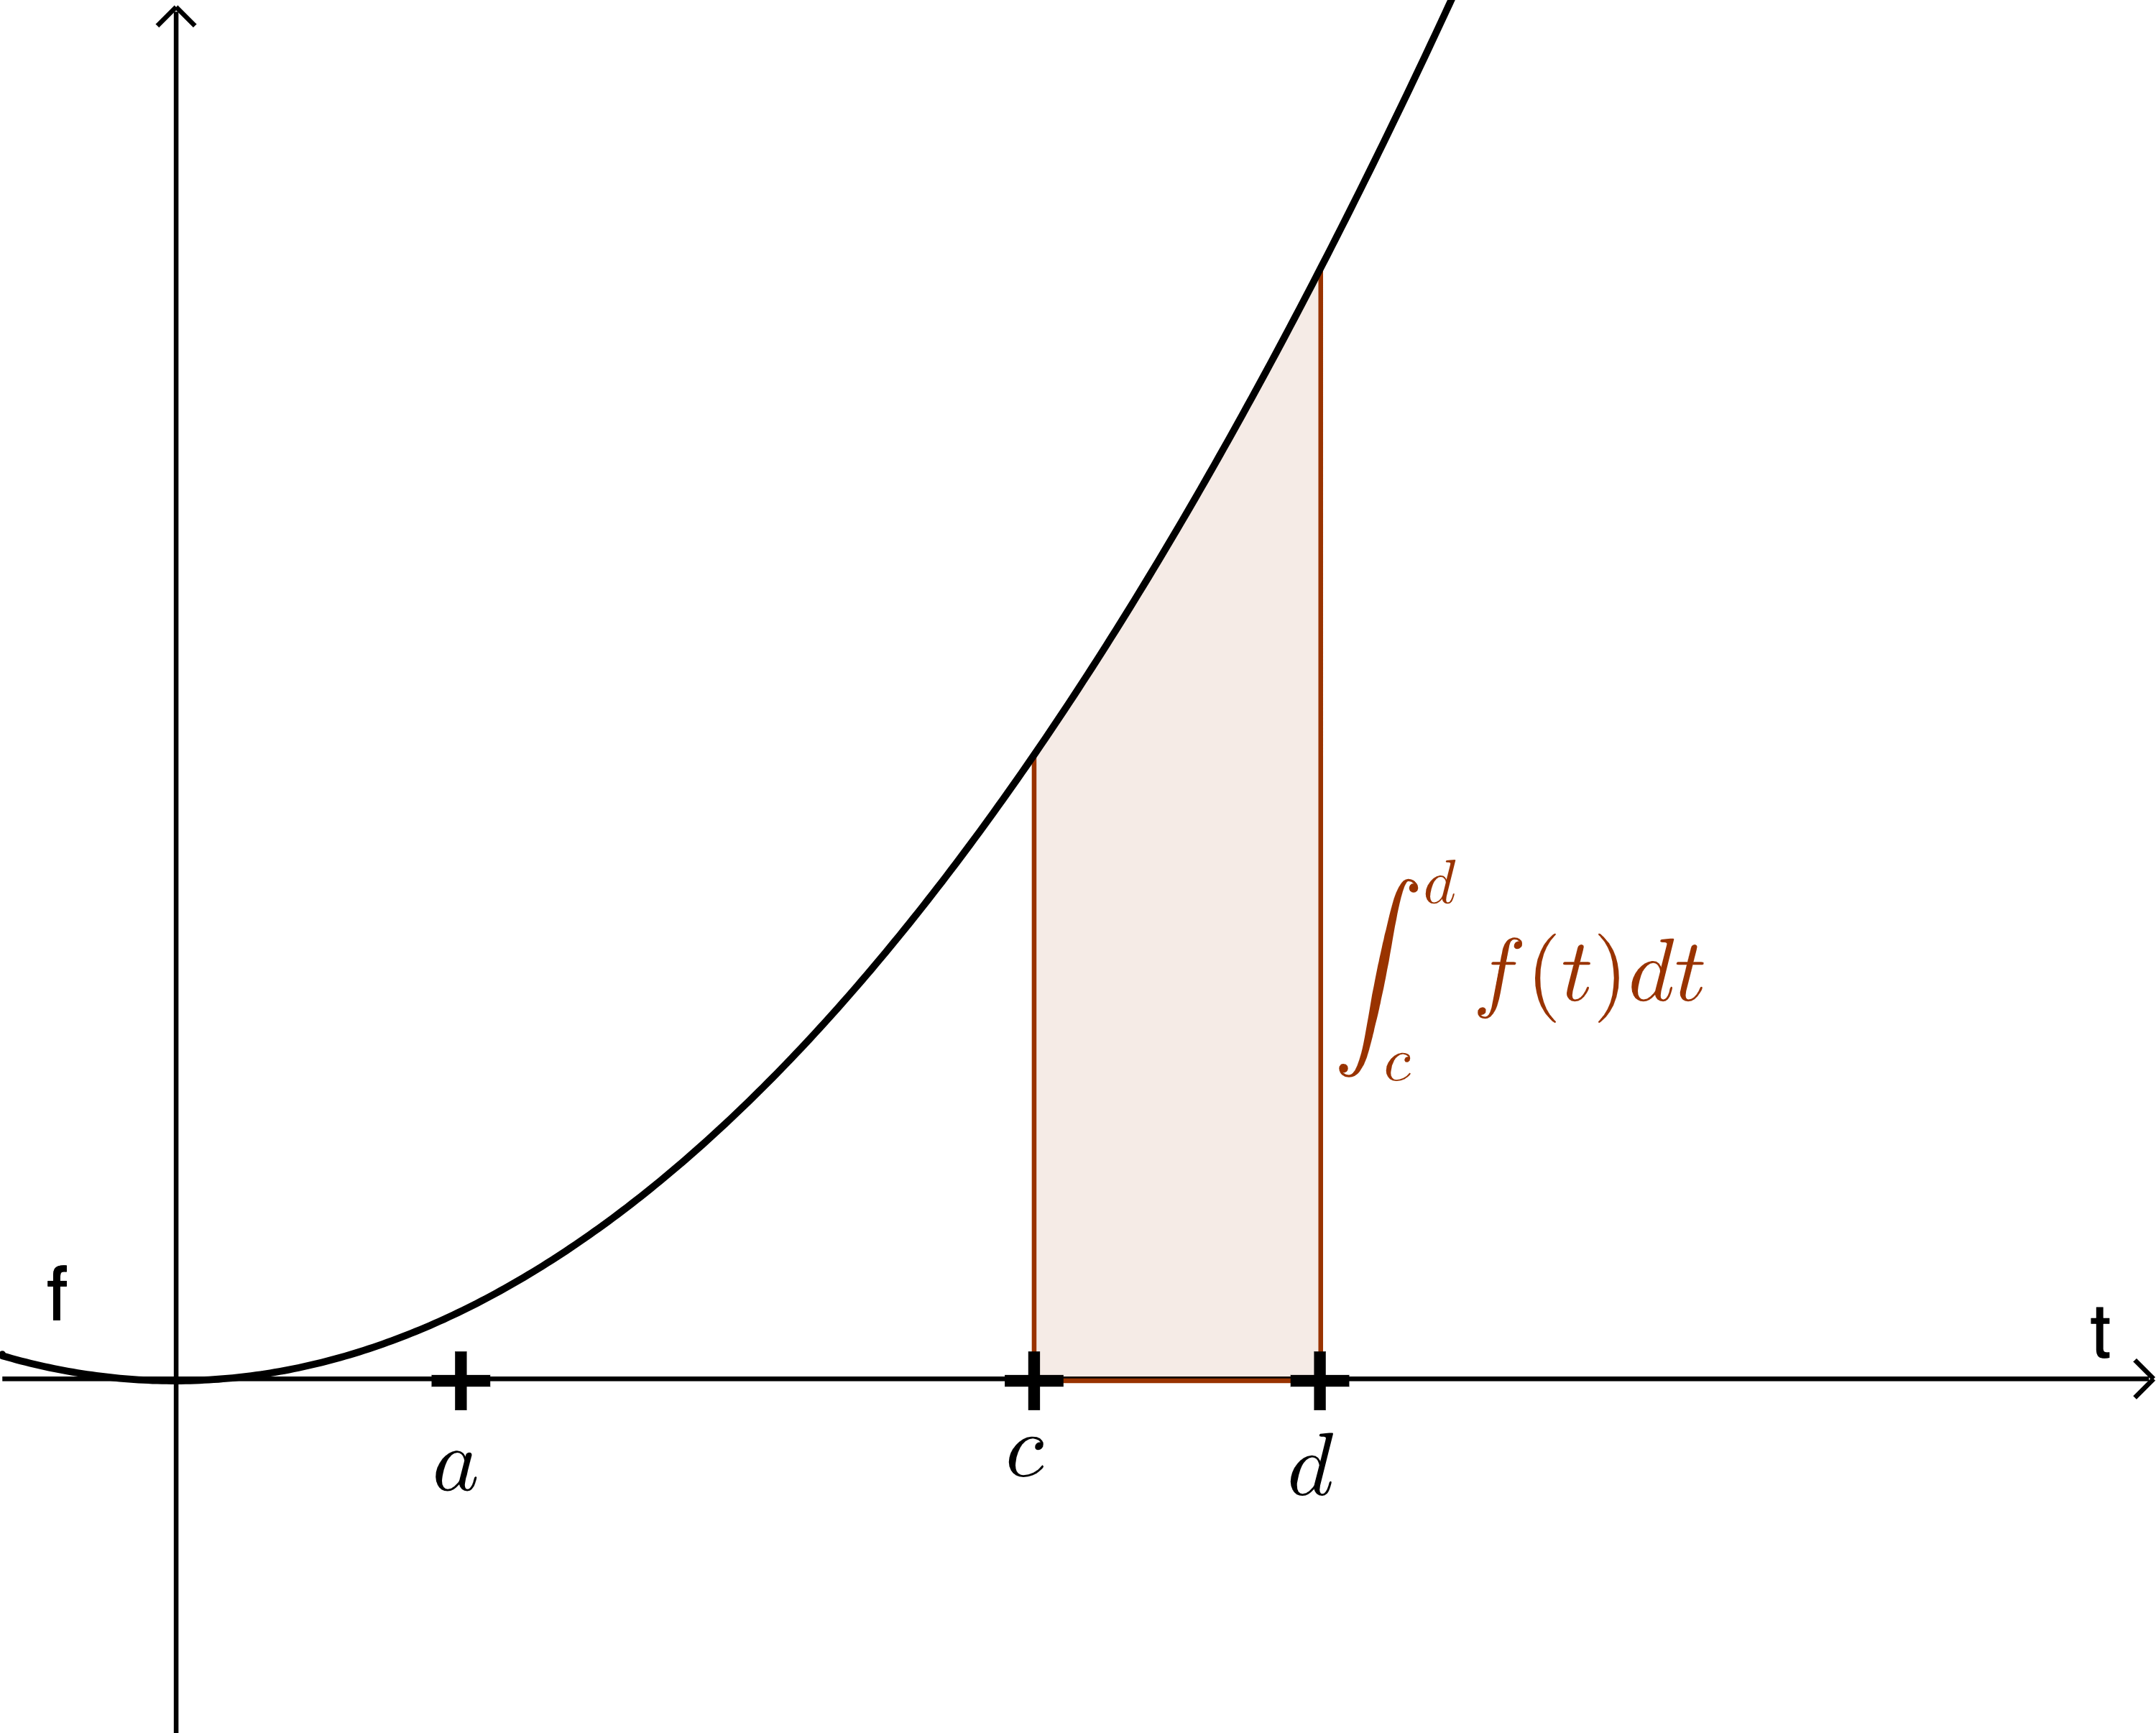
\includegraphics[width=\linewidth]{media/intcd.png}
	\endminipage\hfill
	\minipage{0.32\textwidth}
	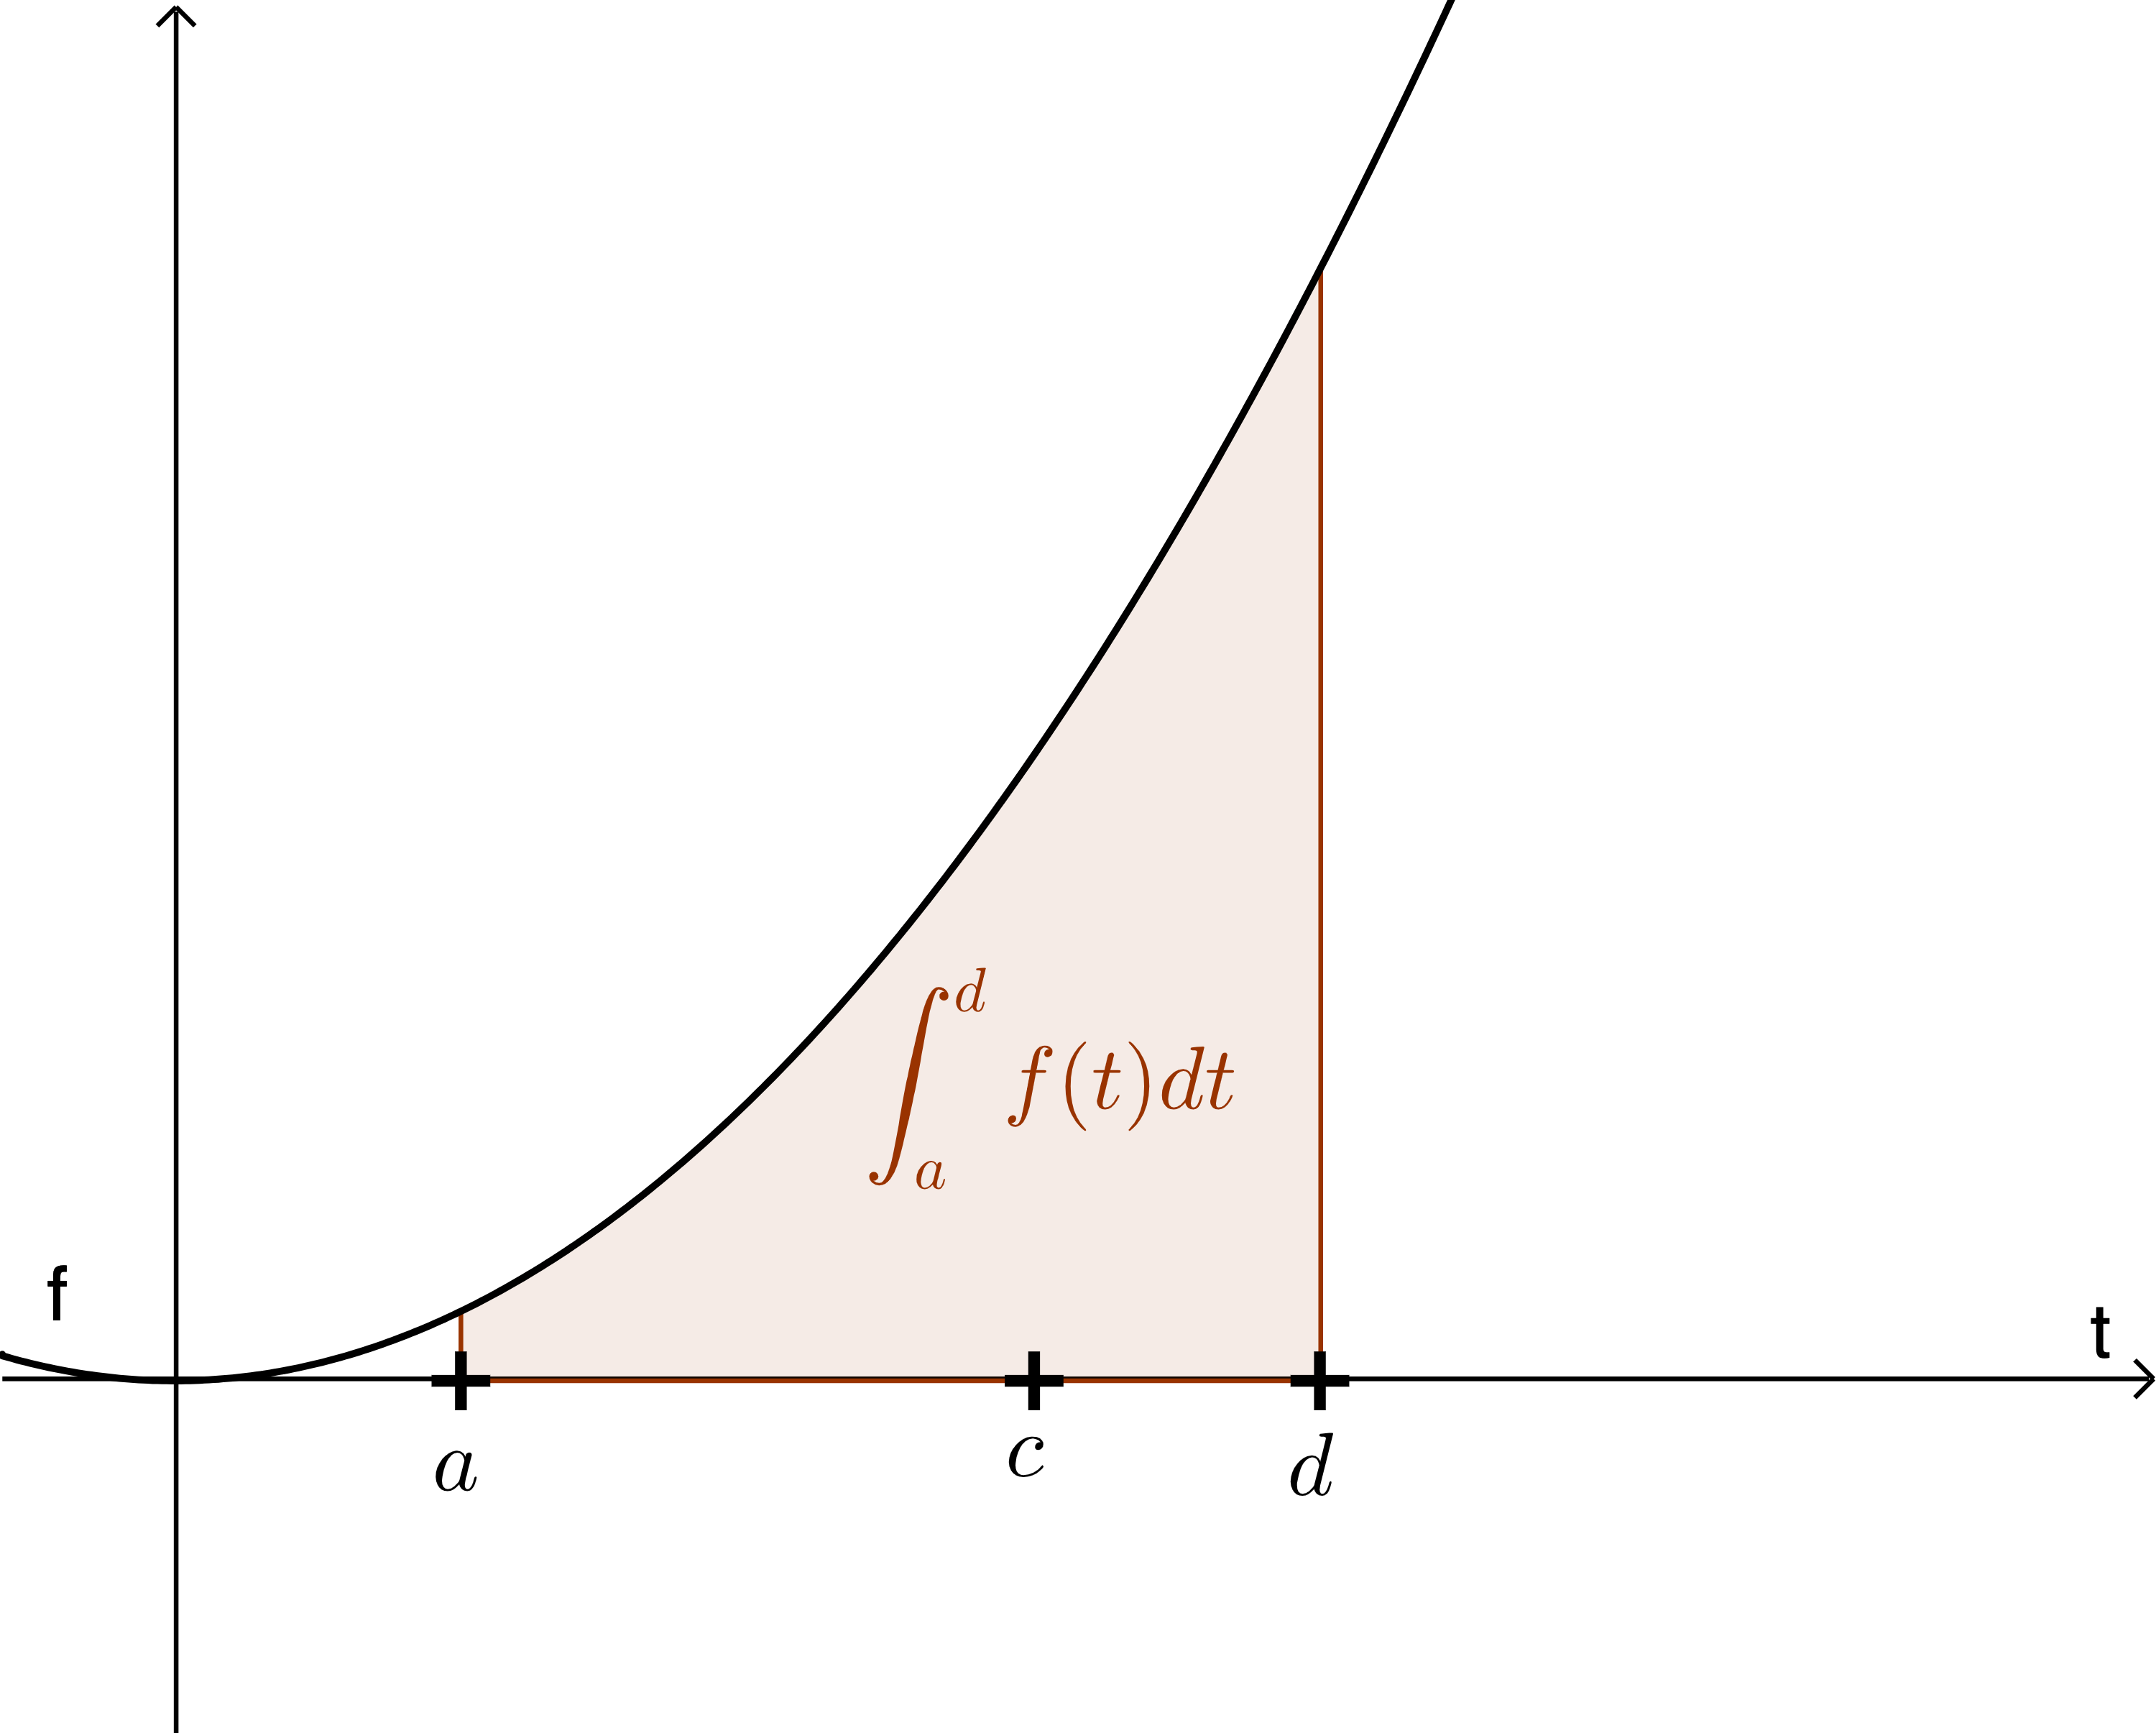
\includegraphics[width=\linewidth]{media/intd.png}
	\endminipage\hfill
	\minipage{0.32\textwidth}
	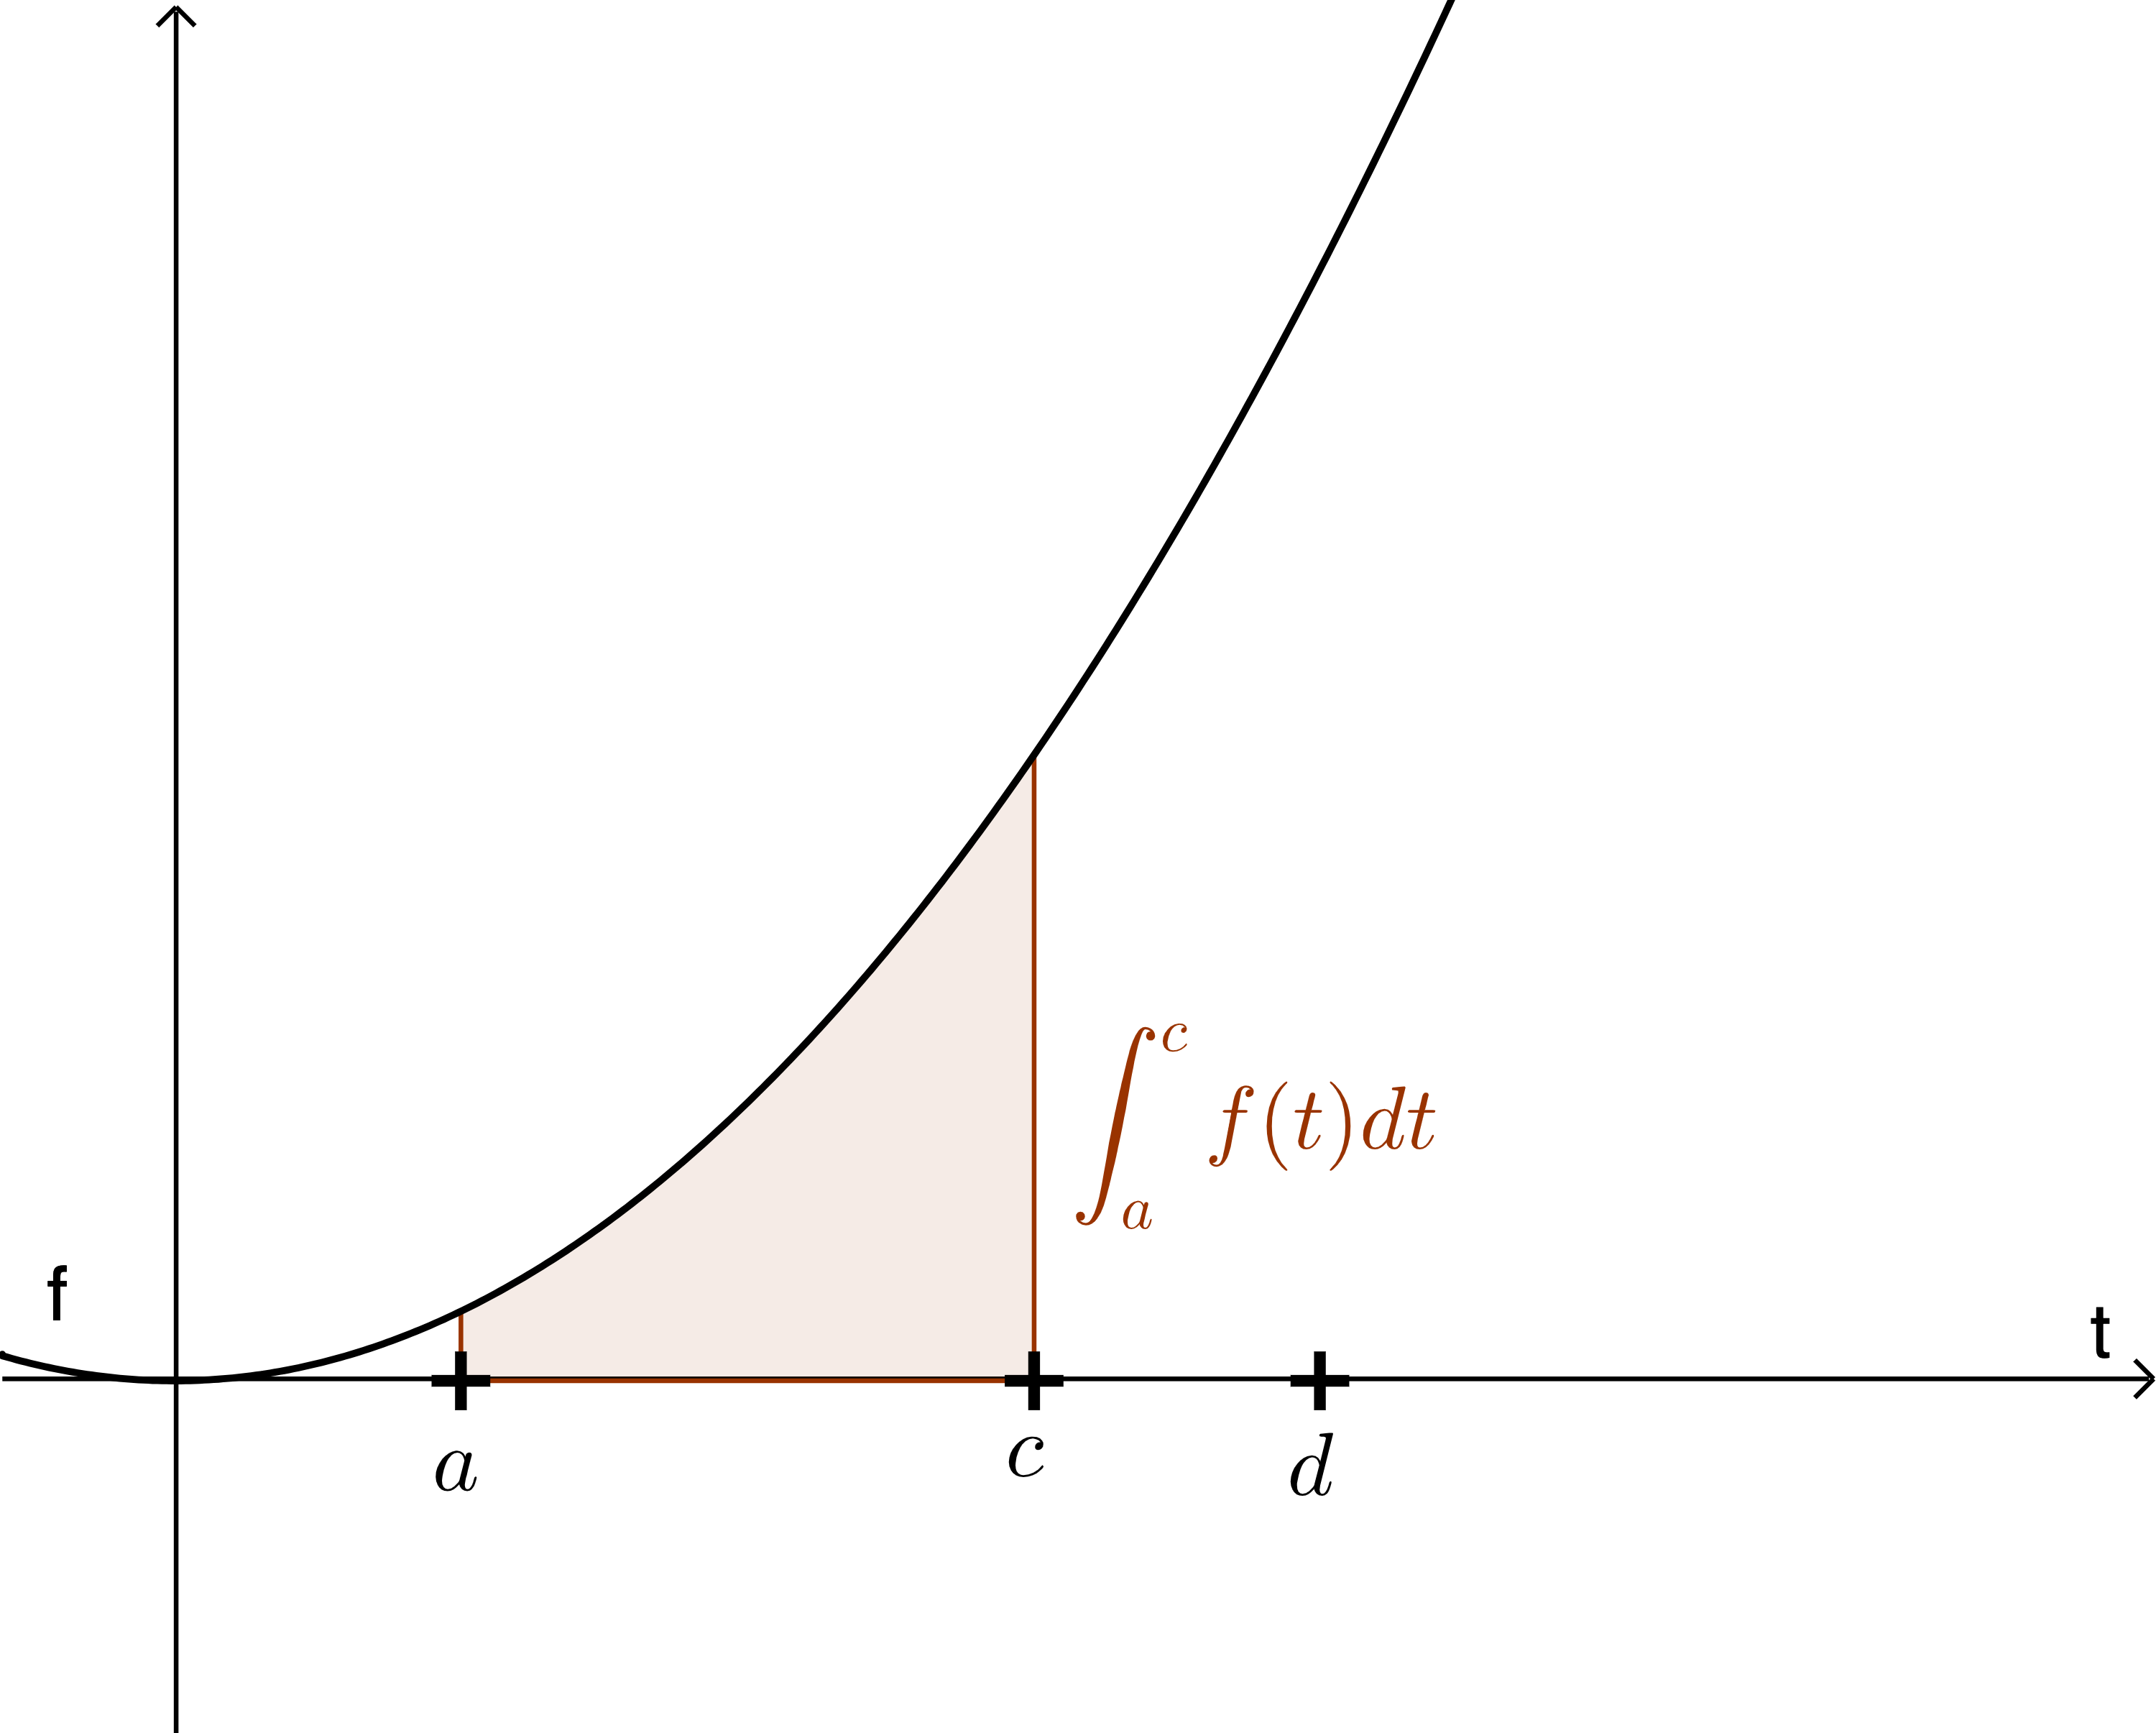
\includegraphics[width=\linewidth]{media/intac.png}
	\endminipage
\end{figure}





Es bleibt die Frage, ob es einen einfachen Weg gibt, eine Integralfunktion einer gegebenen Funktion $f$ zu bestimmen, ohne die Ober- und Untersumme zu berechnen.

\begin{satz}
	{Hauptsatz der Differential- und Integralrechnung}{Hauptsatz}
	Sei $f: \: [a,b] \rightarrow \R$ eine stetige Funktion. Sei $F_a(b)=\int_a^b f(x) \,dx$ eine Integralfunktion von $f$. Dann gilt:
	$$ \frac{d}{dx} F_a(x) = f(x) $$
	Kurz: Integralfunktionen sind Stammfunktionen von $f$.
\end{satz}
\textbf{Bemerkungen}
\begin{enumerate}
	\item Integralfunktionen von $f$ sind nach dem Hauptsatz Stammfunktionen von $f$.
	\item Zu einer gegebenen Funktion gibt es unendliche viele Stammfunktionen. Diese unterscheiden sich durch einen konstanten Summanden.
	\item Aus 1. und 2. folgt: Sei $F(x)$ eine beliebige Stammfunktion von $f$ und $F_0(x)$ die Integralfunktion von $f$ zur unteren Grenze $0$. Dann gibt es eine Konstante $c\in \R$ mit
	      $$F_0(x)=F(x)+c$$
	\item Folglich gilt für die bestimmten Integrale
	      $$ \int_{a}^{b} f(t) \, dt = F_0(b) - F_0(a) = \left(F(b)+c\right)-\left(F(a)+c\right) = F(b) -F(a) $$
\end{enumerate}

\begin{satz}
	{Berechnung von bestimmten Integralen}{}
	Sei $f: \: [a,b] \rightarrow \R$ eine stetige Funktion. Sei $F$ eine \textbf{beliebige} Stammfunktion von $f$. Dann gilt:
	$$ \int_{a}^{b} f(x) \, dx = F(b) -F(a) $$

	Notation: Für $F(b) -F(a)$ schreibt man häufig $\left[F(x)\right]_a^b$
\end{satz}
\begin{bsp}
	{Berechnung eines bestimmten Integrals}{}
	$$\int_1^2 \left(\frac{1}{4} x^2+x+2\right) \, dx=?$$

	Bestimme eine Stammfunktion (anti-Differenzieren): $F(x)=\frac{1}{12}x^3+\frac{1}{2}x^2+2x$.

	Dann folgt
	\begin{align*}
		\int_1^2 \left(\frac{1}{4} x^2+x+2\right) \, dx & =\left[\frac{1}{12}x^3+\frac{1}{2}x^2+2x\right]_1^2                                                          \\
		                                                & = \left(\frac{1}{12}2^3+\frac{1}{2}2^2+2\cdot 2\right) -\left(\frac{1}{12}1^3+\frac{1}{2}1^2+2\cdot 1\right) \\
		                                                & = \frac{49}{12}
	\end{align*}
	\begin{center}
		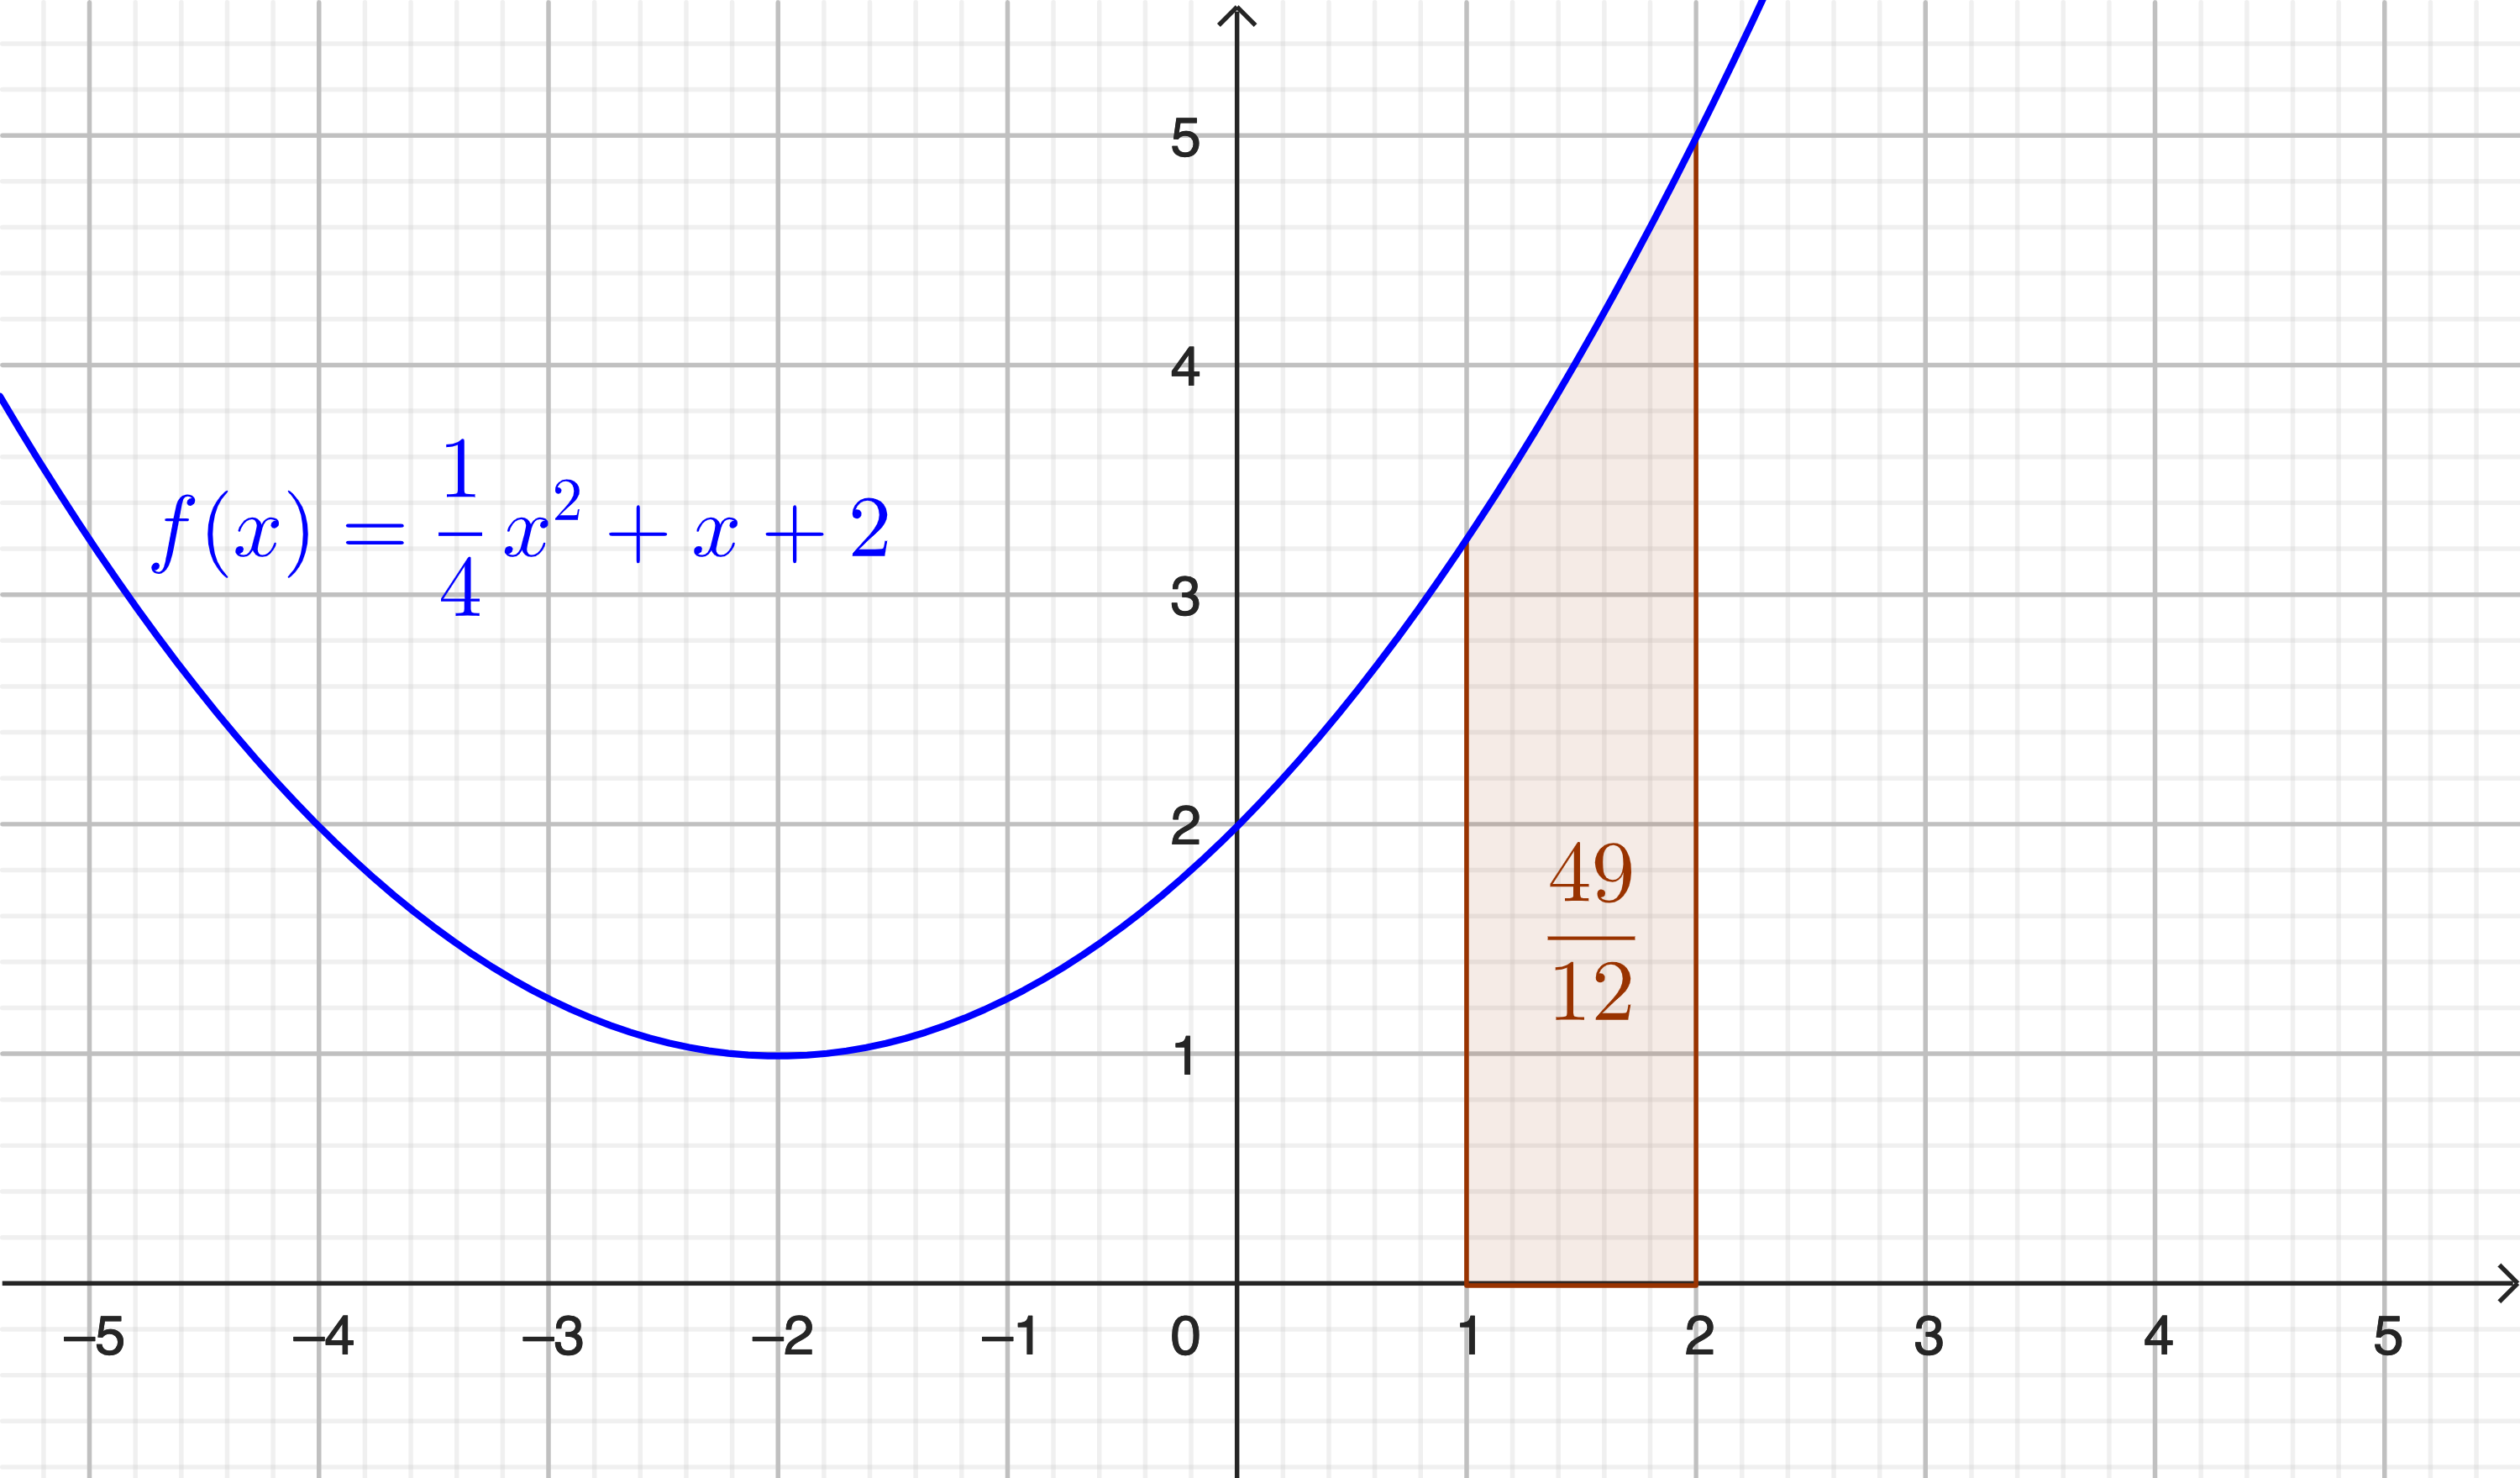
\includegraphics[width = 0.8 \textwidth]{media/bspHauptsatz.png}
	\end{center}
\end{bsp}
\begin{proof}[Beweis des Hauptsatzes der Differential- und Integralrechnung]
	Beim Bestimmen der Ableitung der Integralfunktion $F_a$ helfen uns keine Ableitungsregeln. Wir müssen auf die Definition der Ableitung zurückgreifen.
	Zur Erinnerung: Die Ableitung einer Funktion $f$ ist definiert durch den Differenzialquotienten:
	$$ \frac{d}{dx} f(x)=\lim_{h\rightarrow0} \frac{f(x+h)-f(x)}{h}$$
	Angewendet auf unsere Integralfunktion heisst das:
	$$ \frac{d}{dx} F_a(x)=\lim_{h\rightarrow0} \frac{F_a(x+h)-F_a(x)}{h}$$

	Für die folgenden Überlegungen gehen wir davon aus, dass $h>0$ ist. Der Fall $h<0$ geht analog.

	Schauen wir uns den Zähler $F_a(x+h)-F_a(x)$ etwas genauer an: Er entspricht dem Flächeninhalt der schraffierten Figur:
	\begin{center}
		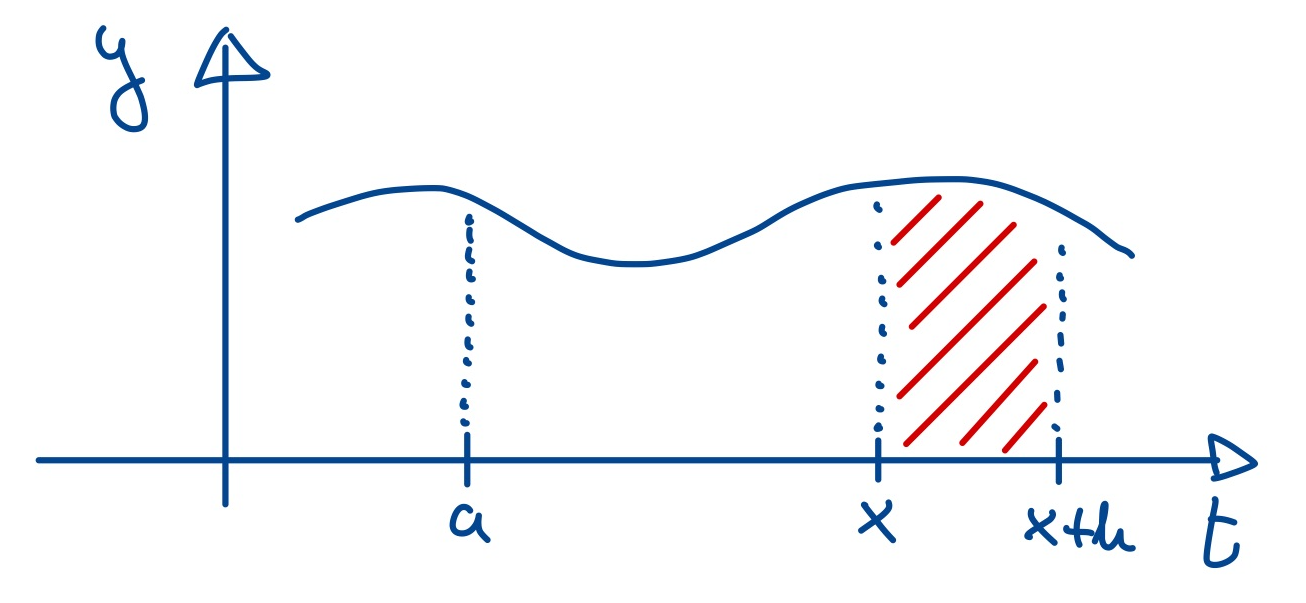
\includegraphics[width = 0.5 \textwidth]{media/BewHauptsatz1.png}
	\end{center}

	Dieser Flächeninhalt können wir nun von oben und von unten durch Rechtecke abschätzen:

	\begin{figure}[!htb]
		\minipage{0.4\textwidth}
		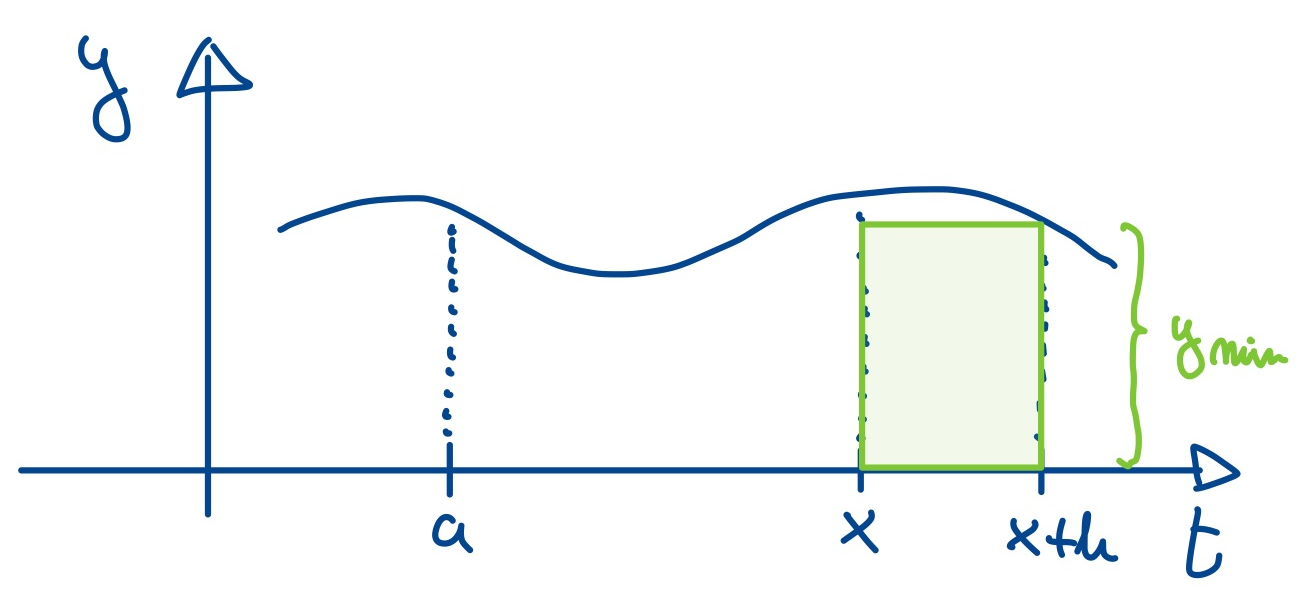
\includegraphics[width=\linewidth]{media/BewHauptsatz2.png}
		\endminipage\hfill
		\minipage{0.4\textwidth}
		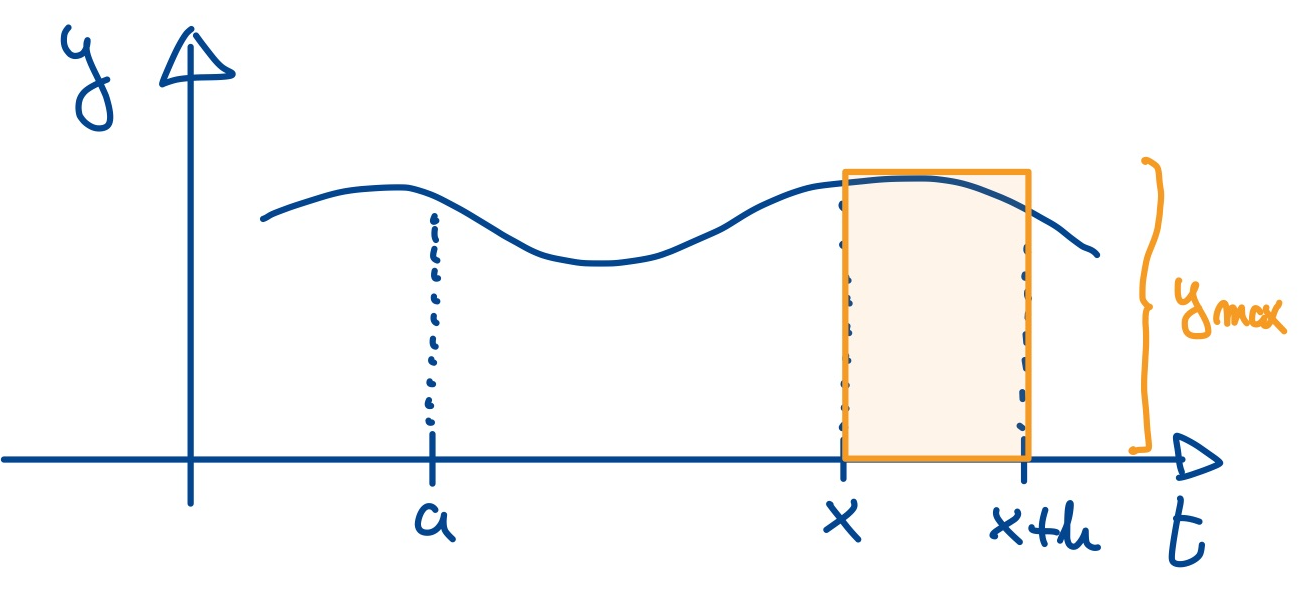
\includegraphics[width=\linewidth]{media/BewHauptsatz3.png}
		\endminipage
	\end{figure}

	Wobei $y_{\text{min}}$  und $y_{\text{max}}$  der kleinste, bzw. grösste Wert von $f(t)$ im Intervall $[x,x+h]$ sind.
	Daraus folgt die Ungleichung
	$$h\cdot y_{\text{min}}\le F_a (x+h)-F_a (x)\le h\cdot y_{\text{max}}$$
	Indem wir beide Seiten der Ungleichung durch $h$ teilen erhalten wir
	$$ y_{\text{min}}\le \frac{F_a (x+h)-F_a (x)}{h}\le y_{\text{max}}$$

	Lassen wir nun $h$ gegen Null streben. Wenn das Intervall $[x,x+h]$ immer kleiner wird, nähert sich der kleinste Wert $y_{\text{min}}$ immer mehr dem Funktionswert $f(x)$. Analog strebt $y_{\text{max}}$ nach $f(x)$. Der mittlere Term $\frac{F_a (x+h)-F_a (x)}{h}$ entspricht für $h \rightarrow0$ genau der Ableitung von $F_a$. Somit gilt:
	$$f(x)\le \frac{d}{dx} F_a (x)\le f(x)$$
	Daraus folgt
	$$\frac{d}{dx} F_a (x)= f(x)$$

\end{proof}

\clearpage
\begin{ueb}
	{}{}
	\begin{enumerate}
		\item Berechnen Sie mit dem Hauptsatz das bestimmte Integral und vergleichen Sie die Ergebnisse. Erklären Sie das Gefundene mithilfe von Skizzen/Geogebra.
		      \begin{enumerate}
			      \item \(\displaystyle \int_0^2 x^2 \, dx \) vergleichen mit:
			            \begin{enumerate}
				            \item \(\displaystyle \int_0^2 (x^2 + 1) \, dx \)
				            \item \(\displaystyle \int_0^2 (x + 1)^2 \, dx \)
				            \item \(\displaystyle \int_{-1}^1 (x + 1)^2 \, dx \)
			            \end{enumerate}
			      \item \(\displaystyle \int_0^4 \sqrt{x} \, dx \) vergleichen mit:
			            \begin{enumerate}
				            \item \(\displaystyle \int_0^4 \sqrt{x + 1} \, dx \)
				            \item \(\displaystyle \int_{-1}^3 \sqrt{x + 1} \, dx \)
				            \item \(\displaystyle \int_1^5 \sqrt{x - 1} \, dx \)
			            \end{enumerate}
		      \end{enumerate}
		\item \textbf{Polynomfunktionen}
		      \begin{enumerate}
			      \item \(\displaystyle \int_0^2 4x^3 \, dx \)
			      \item \(\displaystyle \int_2^4 \frac{1}{5}x^3 \, dx \)
			      \item \(\displaystyle \int_{-1}^2 (x^2 + 3) \, dx \)
			      \item \(\displaystyle \int_3^5 \left( \frac{1}{2}x - 2 \right) \, dx \)
			      \item \(\displaystyle \int_0^3 2x(1 - x) \, dx \)
			      \item \(\displaystyle \int_{-3}^3 (x - 1)^2 \, dx \)
		      \end{enumerate}

		\item \textbf{Gebrochenrationale Funktionen} (Tipp: $\left(\ln(x)\right)'= \frac{1}{x}$)
		      \begin{enumerate}
			      \item \(\displaystyle \int_2^4 \frac{1}{x^2} \, dx \)
			      \item \(\displaystyle \int_{-1}^{-0.5} \frac{3}{x^5} \, dx \)
			      \item \(\displaystyle \int_1^2 \left( 2x - \frac{2}{x} \right) \, dx \)
			      \item \(\displaystyle \int_1^3 \left( 4x - \frac{3}{x} + \frac{2}{x^2} \right) \, dx \)
			      \item \(\displaystyle \int_3^5 \frac{x - 2}{x} \, dx \)
			      \item \(\displaystyle \int_2^3 \frac{x^2 + 4x + 3}{x} \, dx \)
		      \end{enumerate}

		\item \textbf{Wurzelfunktionen}
		      \begin{enumerate}
			      \item \(\displaystyle \int_1^4 3\sqrt{x} \, dx \)
			      \item \(\displaystyle \int_1^4 \frac{1}{\sqrt{x}} \, dx \)
			      \item \(\displaystyle \int_0^8 \sqrt[3]{x} \, dx \)
			      \item \(\displaystyle \int_0^1 x\sqrt{x} \, dx \)
			      \item \(\displaystyle \int_1^4 (2x + 6\sqrt{x}) \, dx \)
			      \item \(\displaystyle \int_1^4 \sqrt{\frac{3}{x^3}} \, dx \)
		      \end{enumerate}

		\item \textbf{Winkelfunktionen}
		      \begin{enumerate}
			      \item \(\displaystyle \int_0^{\frac{\pi}{2}} \sin(t) \, dt \)
			      \item \(\displaystyle \int_\pi^{2\pi} \cos(t) \, dt \)
			      \item \(\displaystyle \int_0^{\frac{\pi}{3}} -2\sin(t) \, dt \)
			      \item \(\displaystyle \int_0^{\pi} (4\sin(t) - 3\cos(t)) \, dt \)
			            % \item \(\displaystyle \int_0^{\frac{7\pi}{4}} \frac{1}{\cos^2(t)} \, dt \)
			            % \item \(\displaystyle \int_{\frac{3\pi}{4}}^{\frac{5\pi}{4}} \tan(t) \, dt \)
		      \end{enumerate}

		\item \textbf{Exponentialfunktionen}
		      \begin{enumerate}
			      \item \(\displaystyle \int_{-1}^1 e^{x+1} \, dx \)
			      \item \(\displaystyle \int_{-1}^0 (2x - e^x) \, dx \)
			      \item \(\displaystyle \int_0^1 \pi \cdot e^x \, dx \)
			      \item \(\displaystyle \int_0^2 (e^x - x^e) \, dx \)
			      \item \(\displaystyle \int_1^2 \left(e^x + \frac{1}{x}\right) \, dx \)
			            % \item \(\displaystyle \int_0^1 10^x \, dx \)
		      \end{enumerate}

		\item \textbf{Einfache Substitutionsregel}
		      \begin{enumerate}
			      \item \(\displaystyle \int_2^5 (2x - 3)^4 \, dx \)
			      \item \(\displaystyle \int_0^6 (5 - 2x)^3 \, dx \)
			      \item \(\displaystyle \int_2^3 \frac{4}{(1 - x)^2} \, dx \)
			      \item \(\displaystyle \int_0^{\frac{\pi}{2}} \sin(3t) \, dt \)
			      \item \(\displaystyle \int_{-\frac{3}{4}}^{\frac{3}{4}} \cos(\pi t) \, dt \)
			      \item \(\displaystyle \int_0^\pi \left(\frac{1}{\pi} + \cos(-2t)\right) \, dt \)
			      \item \(\displaystyle \int_{1/2}^5 \frac{2}{3} e^{4x} \, dx \)
			      \item \(\displaystyle \int_0^6 e^{6 - x} \, dx \)
			      \item \(\displaystyle \int_{-\pi}^\pi (e^x - e^{-x}) \, dx \)
			      \item \(\displaystyle \int_{12}^{24} \frac{1}{\sqrt{2x + 1}} \, dx \)
			      \item \(\displaystyle \int_2^5 \frac{9}{3x - 5} \, dx \)
			            %\item \(\displaystyle \int_{-3}^0 \ln(2) \cdot 2^{-\frac{1}{3}x} \, dx \)
		      \end{enumerate}


	\end{enumerate}

\end{ueb}


\clearpage
\emph{Lösungen}

\begin{enumerate}
	\item Vergleichen der Resultate
	      \begin{enumerate}
		      \item
		            \[
			            \int_0^2 x^2 \, dx
			            = \left[\frac{1}{3}x^3\right]_0^2
			            = \frac{8}{3}
		            \]
		            \begin{enumerate}
			            \item
			                  \[
				                  \int_0^2 (x^2+1)\,dx
				                  = \left[\frac{1}{3}x^3+x\right]_0^2
				                  = 8/3 + 2
				                  = \frac{14}{3}
			                  \]
			            \item
			                  \[
				                  \int_0^2 (x+1)^2\,dx
				                  = \left[\frac{1}{3}x^3+x^2+x\right]_0^2
				                  = \frac{26}{3}
			                  \]
			            \item
			                  \[
				                  \int_{-1}^1 (x+1)^2\,dx
				                  = \left[\frac{1}{3}x^3+x^2+x\right]_{-1}^1
				                  = \frac{8}{3}
			                  \]
		            \end{enumerate}

		      \item
		            \[
			            \int_0^4 \sqrt{x}\,dx
			            = \left[\frac{2}{3}x^{3/2}\right]_0^4
			            = \frac{16}{3}
		            \]
		            \begin{enumerate}
			            \item
			                  \[
				                  \int_0^4 \sqrt{x+1}\,dx
				                  = \left[\frac{2}{3}(x+1)^{3/2}\right]_0^4
				                  = \frac{10\sqrt{5}}{3}-\frac{2}{3}
			                  \]
			            \item
			                  \[
				                  \int_{-1}^3 \sqrt{x+1}\,dx
				                  = \left[\frac{2}{3}(x+1)^{3/2}\right]_{-1}^3
				                  = \frac{16}{3}
			                  \]
			            \item
			                  \[
				                  \int_1^5 \sqrt{x-1}\,dx
				                  = \left[\frac{2}{3}(x-1)^{3/2}\right]_1^5
				                  = \frac{16}{3}
			                  \]
		            \end{enumerate}
	      \end{enumerate}

	\item Polynomfunktionen
	      \begin{enumerate}
		      \item
		            \[
			            \int_0^2 4x^3\,dx
			            = \left[x^4\right]_0^2
			            = 16
		            \]
		      \item
		            \[
			            \int_2^4 \frac{1}{5}x^3\,dx
			            = \left[\frac{1}{20}x^4\right]_2^4
			            = 12
		            \]
		      \item
		            \[
			            \int_{-1}^2 (x^2+3)\,dx
			            = \left[\frac{1}{3}x^3+3x\right]_{-1}^2
			            = 12
		            \]
		      \item
		            \[
			            \int_3^5 \left(\frac{1}{2}x-2\right)\,dx
			            = \left[\frac{1}{4}x^2-2x\right]_3^5
			            = 0
		            \]
		      \item
		            \[
			            \int_0^3 2x(1-x)\,dx
			            = \left[x^2-\frac{2}{3}x^3\right]_0^3
			            = -9
		            \]
		      \item
		            \[
			            \int_{-3}^3 (x-1)^2\,dx
			            = \int_{-3}^3 (x^2-2x+1) \,dx
			            = \left[\frac{1}{3}x^3-x^2+x\right]_{-3}^3
			            = 24
		            \]
	      \end{enumerate}

	\item Gebrochenrationale Funktionen
	      \begin{enumerate}
		      \item
		            \[
			            \int_2^4 \frac{1}{x^2}\,dx
			            =  \int_2^4 x^{-2}\,dx
			            = \left[-x^{-1}\right]_2^4
			            = \frac{1}{4}
		            \]
		      \item
		            \[
			            \int_{-1}^{-0.5} \frac{3}{x^5}\,dx
			            = \left[-\frac{3}{4}x^{-4}\right]_{-1}^{-0.5}
			            = -11.25
		            \]
		      \item
		            \[
			            \int_1^2 \left(2x-\frac{2}{x}\right)\,dx
			            = \left[x^2-2\ln(x)\right]_1^2
			            = 3-2\ln(2)\approx 1.61
		            \]
		      \item
		            \[
			            \int_1^3 \left(4x-\frac{3}{x}+\frac{2}{x^2}\right)\,dx
			            = \left[2x^2-3\ln(x)-\frac{2}{x}\right]_1^3
			            = \frac{52}{3}-3\ln(3)\approx 14.04
		            \]
		      \item
		            \[
			            \int_3^5 \frac{x-2}{x}\,dx
			            = \int_3^5 \left(1-2\cdot\frac{1}{x}\right)\,dx
			            = \left[x-2\ln(x)\right]_3^5
			            = 2\ln\!\left(\frac{3}{5}\right)+2 \approx 0.98
		            \]
		      \item
		            \[
			            \int_2^3 \frac{x^2+4x+3}{x}\,dx
			            = \left[\frac{1}{2}x^2+4x+3\ln(x)\right]_2^3
			            = 3\ln\!\left(\frac{3}{2}\right)+\frac{13}{2}\approx 7.72
		            \]
	      \end{enumerate}

	\item Wurzelfunktionen
	      \begin{enumerate}
		      \item
		            \[
			            \int_1^4 3\sqrt{x}\,dx
			            =  \int_1^4 3 x^{1/2}\,dx
			            = \left[2x^{3/2}\right]_1^4
			            = 14
		            \]
		      \item
		            \[
			            \int_1^4 \frac{1}{\sqrt{x}}\,dx
			            = \int_1^4 x^{-1/2}\,dx
			            = \left[2\sqrt{x}\right]_1^4
			            = 2
		            \]
		      \item
		            \[
			            \int_0^8 \sqrt[3]{x}\,dx
			            = \int_0^8 x^{1/3}\,dx
			            = \left[\frac{3}{4}x^{4/3}\right]_0^8
			            = 12
		            \]
		      \item
		            \[
			            \int_0^1 x\sqrt{x}\,dx
			            = \int_0^1 x^{3/2}\,dx
			            = \left[\frac{2}{5}x^{5/2}\right]_0^1
			            = \frac{2}{5}
		            \]
		      \item
		            \[
			            \int_1^4 (2x+6\sqrt{x})\,dx
			            = \left[x^2+4x^{3/2}\right]_1^4
			            = 43
		            \]
		      \item
		            \[
			            \int_1^4 \sqrt{\frac{3}{x^3}}\,dx
			            = \int_1^4 \sqrt{3}\cdot x^{-3/2}\,dx
			            = \left[\sqrt{3}\cdot (-2)\cdot x^{-1/2}\right]_1^4
			            = \sqrt{3}
		            \]
	      \end{enumerate}

	\item Winkelfunktionen
	      \begin{enumerate}
		      \item
		            \[
			            \int_0^{\frac{\pi}{2}} \sin(t)\,dt
			            = \left[-\cos(t)\right]_0^{\frac{\pi}{2}}
			            = 1
		            \]
		      \item
		            \[
			            \int_\pi^{2\pi} \cos(t)\,dt
			            = \left[\sin(t)\right]_\pi^{2\pi}
			            = 0
		            \]
		      \item
		            \[
			            \int_0^{\frac{\pi}{3}} -2\sin(t)\,dt
			            = \left[2\cos(t)\right]_0^{\frac{\pi}{3}}
			            = -1
		            \]
		      \item
		            \[
			            \int_0^{\pi} (4\sin(t)-3\cos(t))\,dt
			            = \left[-4\cos(t)-3\sin(t)\right]_0^{\pi}
			            = 8
		            \]
	      \end{enumerate}

	\item Exponentialfunktionen
	      \begin{enumerate}
		      \item
		            \[
			            \int_{-1}^ 1 e\cdot e^{x}\,dx
			            = \left[ e \cdot e^{x}\right]_{-1}^1
			            = e^2-1
		            \]
		      \item
		            \[
			            \int_{-1}^0 (2x-e^x)\,dx
			            = \left[x^2-e^x\right]_{-1}^0
			            = \frac{1}{e}-2
		            \]
		      \item
		            \[
			            \int_0^1 \pi\cdot e^x\,dx
			            = \left[\pi e^x\right]_0^1
			            = \pi(e-1)
		            \]
		      \item
		            \[
			            \int_0^2 (e^x-x^e)\,dx
			            = \left[e^x-\frac{1}{e+1}x^{e+1}\right]_0^2
			            \approx 2.85
		            \]
		      \item
		            \[
			            \int_1^2 \left(e^x+\frac{1}{x}\right)\,dx
			            = \left[e^x+\ln(x)\right]_1^2
			            \approx 5.36
		            \]
	      \end{enumerate}

	\item Einfache Substitutionsregel
	      \begin{enumerate}
		      \item
		            \[
			            \int_2^5 (2x-3)^4\,dx
			            = \left[\frac{1}{10}(2x-3)^5\right]_2^5
			            = 1680.6
		            \]
		      \item
		            \[
			            \int_0^6 (5-2x)^3\,dx
			            = \left[-\frac{1}{8}(5-2x)^4\right]_0^6
			            = -222
		            \]
		      \item
		            \[
			            \int_2^3 \frac{4}{(1-x)^2}\,dx
			            = \left[\frac{4}{1-x}\right]_2^3
			            = 2
		            \]
		      \item
		            \[
			            \int_0^{\frac{\pi}{2}} \sin(3t)\,dt
			            = \left[-\frac{1}{3}\cos(3t)\right]_0^{\frac{\pi}{2}}
			            = \frac{1}{3}
		            \]
		      \item
		            \[
			            \int_{-\frac{3}{4}}^{\frac{3}{4}} \cos(\pi t)\,dt
			            = \left[\frac{1}{\pi}\sin(\pi t)\right]_{-\frac{3}{4}}^{\frac{3}{4}}
			            = \frac{\sqrt{2}}{\pi}
		            \]
		      \item
		            \[
			            \int_0^\pi \left(\frac{1}{\pi}+\cos(-2t)\right)\,dt
			            = \left[\frac{t}{\pi}-\frac{1}{2}\sin(-2t)\right]_0^\pi
			            = 1
		            \]
		      \item
		            \[
			            \int_{1/2}^5 \frac{2}{3}e^{4x}\,dx
			            = \left[\frac{1}{6}e^{4x}\right]_{1/2}^5
			            = \frac{1}{6}\left(e^{20}-e^2\right)
		            \]
		      \item
		            \[
			            \int_0^6 e^{6-x}\,dx
			            = \left[-e^{6-x}\right]_0^6
			            = e^6-1
		            \]
		      \item
		            \[
			            \int_{-\pi}^{\pi} (e^x-e^{-x})\,dx
			            = \left[e^x+e^{-x}\right]_{-\pi}^{\pi}
			            = 0
		            \]
		      \item
		            \[
			            \int_{12}^{24} \frac{1}{\sqrt{2x+1}}\,dx
			            = \left[\sqrt{2x+1}\right]_{12}^{24}
			            = 2
		            \]
		      \item
		            \[
			            \int_2^5 \frac{9}{3x-5}\,dx
			            = \left[3\ln|3x-5|\right]_2^5
			            = 3\ln(10)
		            \]
	      \end{enumerate}
\end{enumerate}

% \begin{enumerate}
% 	\item Vergleichen der Resultate
% 	      \begin{enumerate}
% 		      \item $8/3$
% 		            \begin{enumerate}
% 			            \item $14/3 = 8/3 + 2$
% 			            \item $26/3$
% 			            \item $8/3$
% 		            \end{enumerate}
% 		      \item $16/3$
% 		            \begin{enumerate}
% 			            \item $\frac{10\sqrt{5}}{3} - \frac{2}{3}$
% 			            \item $16/3$
% 			            \item $16/3$
% 		            \end{enumerate}
% 	      \end{enumerate}

% 	\item Polynomfunktionen
% 	      \begin{enumerate}
% 		      \item 16
% 		      \item 12
% 		      \item 12
% 		      \item 0
% 		      \item -9
% 		      \item 24
% 	      \end{enumerate}

% 	\item Gebrochenrationale Funktionen
% 	      \begin{enumerate}
% 		      \item 1/4
% 		      \item $-11.25$
% 		      \item $3-\ln(2)\approx 1.61$
% 		      \item $\frac{52}{3} - 3\ln(3) \approx 14.04$
% 		      \item $2\ln(3/5) + 2 \approx 0.98$
% 		      \item $3\ln(3/2)+13/2 \approx 7.72$
% 	      \end{enumerate}

% 	\item Wurzelfunktionen
% 	      \begin{enumerate}
% 		      \item 14
% 		      \item 2
% 		      \item 12
% 		      \item 2/5
% 		      \item 43
% 		      \item $\sqrt{3}$
% 	      \end{enumerate}


% 	\item Winkelfunktionen
% 	      \begin{enumerate}
% 		      \item 1
% 		      \item 0
% 		      \item -1
% 		      \item 8
% 		            % \item 1
% 		            % \item $\frac{1}{2} \ln(2)$
% 	      \end{enumerate}

% 	\item Exponentialfunktionen
% 	      \begin{enumerate}
% 		      \item $e^2 -1$
% 		      \item $\frac{1}{e} -2$
% 		      \item $\pi (e-1)$
% 		      \item $\approx 2.85$
% 		      \item $\approx 5.36$
% 		            %\item $\approx 3.91$ 
% 	      \end{enumerate}

% 	\item Einfache Substitutionsregel
% 	      \begin{enumerate}
% 		      \item 1680.6
% 		      \item 0
% 		      \item 2
% 		      \item 1/3
% 		      \item $\sqrt{2} / \pi$
% 		      \item 1
% 		      \item $\frac{1}{6} \left(e^{20}-1\right)$
% 		      \item $e^{12}-1$
% 		      \item 0
% 		      \item 2
% 		      \item $3\ln(10)$
% 		            %\item 3 
% 	      \end{enumerate}
% \end{enumerate}

